\documentclass[a4paper,10pt,russian]{article}
\usepackage[utf8]{inputenc}
\usepackage[russian]{babel}
\usepackage{indentfirst}
\usepackage{amssymb,amsmath}
\usepackage{multicol}
\usepackage{soulutf8}
\usepackage{graphicx}
\usepackage{longtable}
\usepackage{spverbatim}
\usepackage{ucs}
\usepackage{misccorr}
\usepackage{float}
\usepackage{makecell}           % break line in cell
\usepackage{hyperref}

\usepackage{xcolor}
\definecolor{light-gray}{gray}{0.9}
\definecolor{string-gray}{gray}{0.3}

\usepackage{cmap}
\usepackage{pscyr}

\usepackage{listings}           % source code `bl
% "define" Scala
\lstdefinelanguage{scala}{
    morekeywords={abstract,case,catch,class,def, %
      do,else,extends,false,final,finally,       %
      for,if,implicit,import,match,mixin,        %
      new,null,object,override,package,          %
      private,protected,requires,return,sealed,  %
      super,this,throw,trait,true,try,           %
      type,val,var,while,with,yield},
    otherkeywords={=>,<-,<\%,<:,>:,\#,@,::,:+,+:},
    sensitive=true,
    morecomment=[l]{//},
    morecomment=[n]{/*}{*/},
    morestring=[b]",
    morestring=[b]',
    morestring=[b]"""
}

\lstset{
    escapeinside={\#@}{@},
    extendedchars=\true,
    numbers=left,
    inputencoding=utf8,
    keepspaces=true,
    basicstyle=\footnotesize\ttfamily,
    backgroundcolor=\color{light-gray},
    keywordstyle=\bfseries,
    commentstyle=\itshape\color{string-gray},
    stringstyle=\color{string-gray},
    breaklines=true,
    columns=fullflexible,
    tabsize=4
}


\parskip=0pt                % интервал между абзацами

\usepackage{geometry}       % Меняем поля страницы
\geometry{left=1.5cm}         % левое поле
\geometry{right=1.5cm}      % правое поле
\geometry{top=1cm}          % верхнее поле
\geometry{bottom=1.5cm}       % нижнее поле

\begin{document}

\begin{titlepage}
        \newpage
        \begin{large}
                \begin{center}
                        Университет ИТМО\\

                        \vspace{5em}
                        \begin{scshape} Кафедра вычислительной техники \end{scshape}\\

                        \vspace{4em}
                        Лабораторная работа №1\\
                        по тестированию программного обеспечения\\

                        \vspace{1em}
%                        \begin{bfseries}  \end{bfseries}\\
                        Вариант 5
                \end{center}

                \begin{flushright}
                        \vspace{6em}
                        \begin{bfseries} Выполнили: \end{bfseries}\\
                        \begin{itshape}
                                Студент 3-го курса\\
                                гр. P3311\\
                                Томилов Н. А.\\
                                Студент 3-го курса\\
                                гр. P3311\\
                                Киреев В. Ю.\\
                        \end{itshape}

                        \vspace{3em}
                        \begin{bfseries} Преподаватель: \end{bfseries}\\
                        \begin{itshape}
                                Клименков С. В. \\
                        \end{itshape}
                \end{flushright}

                \begin{center}
                        \vspace{\fill}
                        Санкт-Петербург\\
                        2018 г.
                \end{center}
        \end{large}
\end{titlepage}


\setcounter{page}{2}

\section{Часть 1}
\subsection{Постановка задачи}
Для указанной функции провести модульное тестирование разложения функции в степенной ряд. Выбрать достаточное тестовое покрытие.
\subsection{Функция}
Функция $ sin(x) $
\subsection{Исходный код}
\lstinputlisting[language=java]{../src/main/java/testing/lab1/Calculator.java}
\subsection{Тесты}
\lstinputlisting[language=java]{../src/test/java/testing/lab1/CalculatorTest.java}
\subsection{Обоснование тестового покрытия}
Первая группа тестов проверяет, что синус не выходит за пределы $ [-1; 1] $.
Эта группа дополняет следующую, которая демонстрирует, что в примечательных точках
наш синус даёт корректные результаты. На Рис. \ref{f:sin-cover} показано, как
выбраны данные точки.
\begin{figure}[H]
  \centering
  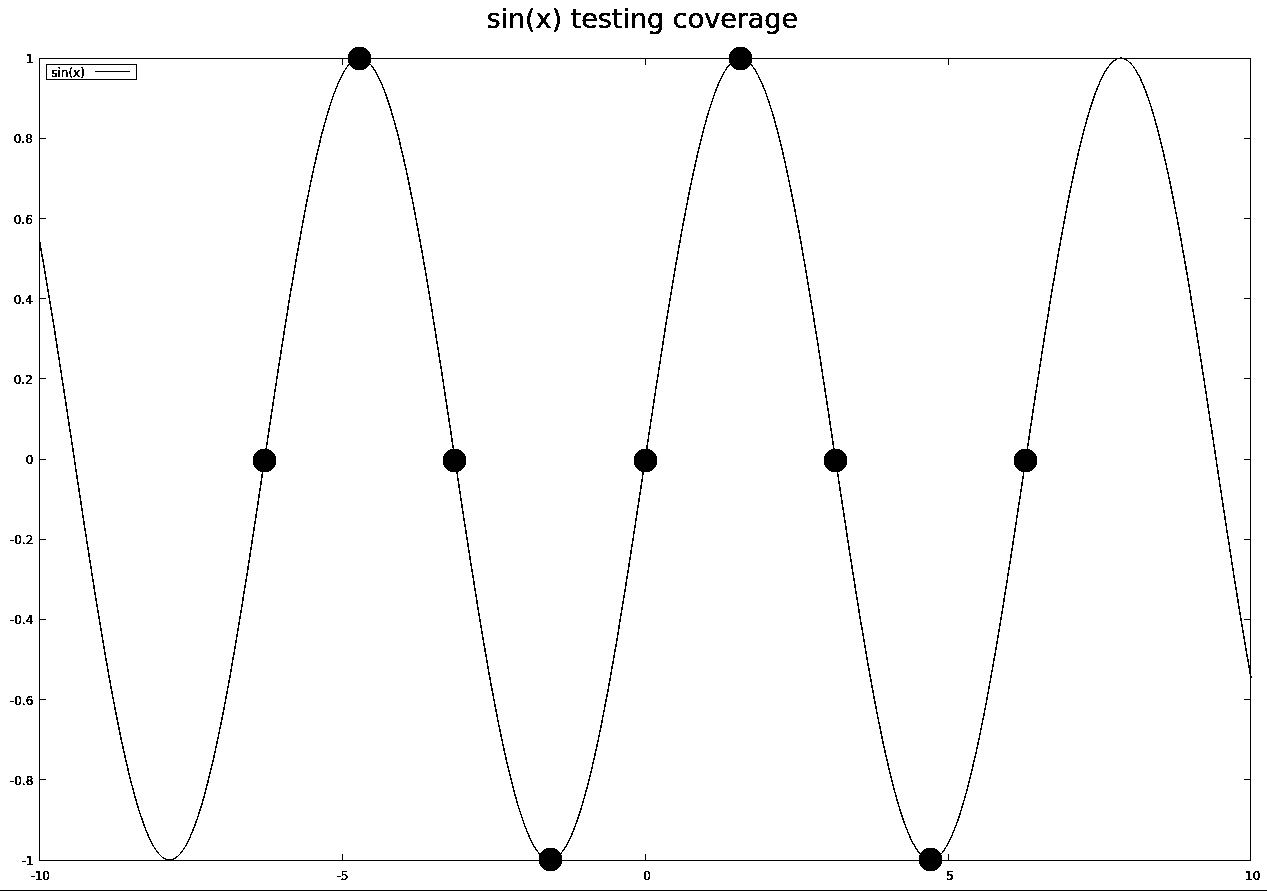
\includegraphics[scale=0.5]{./sin-cover.png}
  \caption{Тестовое покрытие для $ sin(x) $}
  \label{f:sin-cover}
\end{figure}

Таким образом, проверка периодичность появления примечательных точек ( $ -2\pi $,
$ -\frac{3}{2}\pi $, $ -\pi $, $ -\frac{1}{2}\pi $, $ 0 $, $ \frac{1}{2}\pi $,
$ \pi $, $ \frac{3}{2}\pi $, $ 2\pi $) и общее попадание в теоретическое множество
значений функции синуса в рамках, в которых применимо разложение в ряд Тейлора,
позволяет сделать положительный вывод о качестве реализованного алгоритма вычисления
синуса.


\section{Часть 2}
\subsection{Постановка задачи}
Провести модульное тестирование указанного алгоритма. Для этого выбрать характерные точки внутри алгоритма, и для предложенных самостоятельно наборов исходных данных записать последовательность попадания в характерные точки. Сравнить последовательность попадания с эталонной.
\subsection{Алгоритм}
Программный модуль для сортировки массива по алгоритму быстрой сортировки \url{http://www.cs.usfca.edu/~galles/visualization/ComparisonSort.html}
\subsection{Исходный код}
\subsubsection{Сортировка}
\lstinputlisting[language=java]{../src/main/java/testing/lab1/QuickSort.java}
\subsubsection{QsortSwapAction.java}
\begin{lstlisting}[language=java]
package testing.lab1;

public class QsortSwapAction {
    private int pivot;
    private int pivotIndex;

    private int leftValue;
    private int leftIndex;

    private int rightValue;
    private int rightIndex;

    public QsortSwapAction(int pivot, int pivotIndex, int leftValue, int leftIndex, int rightValue, int rightIndex) {
        this.pivot = pivot;
        this.pivotIndex = pivotIndex;
        this.leftValue = leftValue;
        this.leftIndex = leftIndex;
        this.rightValue = rightValue;
        this.rightIndex = rightIndex;
    }

    @Override
    public String toString() {
        return "QsortSwapAction{" +
                "pivot=" + pivot +
                ", pivotIndex=" + pivotIndex +
                ", leftValue=" + leftValue +
                ", leftIndex=" + leftIndex +
                ", rightValue=" + rightValue +
                ", rightIndex=" + rightIndex +
                '}';
    }

    @Override
    public boolean equals(Object o) {
        if (this == o) return true;
        if (o == null || getClass() != o.getClass()) return false;

        QsortSwapAction that = (QsortSwapAction) o;

        if (pivot != that.pivot) return false;
        if (pivotIndex != that.pivotIndex) return false;
        if (leftValue != that.leftValue) return false;
        if (leftIndex != that.leftIndex) return false;
        if (rightValue != that.rightValue) return false;
        return rightIndex == that.rightIndex;
    }
    // getters and setters
}
\end{lstlisting}
\subsubsection{QsortSwapActionHistory.java}
\lstinputlisting[language=java]{../src/main/java/testing/lab1/QsortSwapActionHistory.java}
\subsection{Тесты}
\lstinputlisting[language=java]{../src/test/java/testing/lab1/QuickSortTest.java}
\subsection{Обоснование тестового покрытия}
В сортировку передан объект, позволяющий сохранять историю обменов элементов в массиве.
Первый тест просто сравнивает результаты сортировки с упорядоченным набором.
Следующий проверяет, что на большом массиве алгоритм делает один из необходимых шагов.

Дальнейшие тесты направлены на проверку корректности поведения алгоритма на всех стадиях работы.
Группа тестов \texttt{noActionsTest} проверяет, что для отсортированных массивов
(и, в частности, пустого) не производится никаких действий. Тест \texttt{halfSortedTest}
позволяет отследить, как алгоритм ведёт себя на частично отсортированном массиве.
\texttt{reversedTest} демонстрирует работу на отсортированном в обратном порядке
массиве, который является ещё одним вырожденным случаем для алгоритма, подтверждающим
его корректность. \texttt{npeTest} служит для проверки на уведомление об ошибке
(выбросе исключения) в случае передачи алгоритму значения \texttt{null} вместо
ссылки на массив.

Таким образом удалось покрыть алгоритм адекватным набором тестов, демонстрирующих
его корректную работу как на произвольных данных, так и в вырожденных случаях.


\section{Часть 3}
\subsection{Постановка задачи}
Сформировать доменную модель для заданного текста.  Разработать тестовое покрытие для данной доменной модели.
\subsection{Описание предметной области}
\begin{quote}
	Легко, как балерина, Зафод вскочил на ноги и начал осматриваться. До самого горизонта во все стороны простиралась сплошная золотая поверхность. Она блестела, как... впрочем, этому невозможно подобрать сравнение, потому что ничто во Вселенной не блестит так, как планета из чистого золота.
\end{quote}
\subsection{UML-диаграмма}
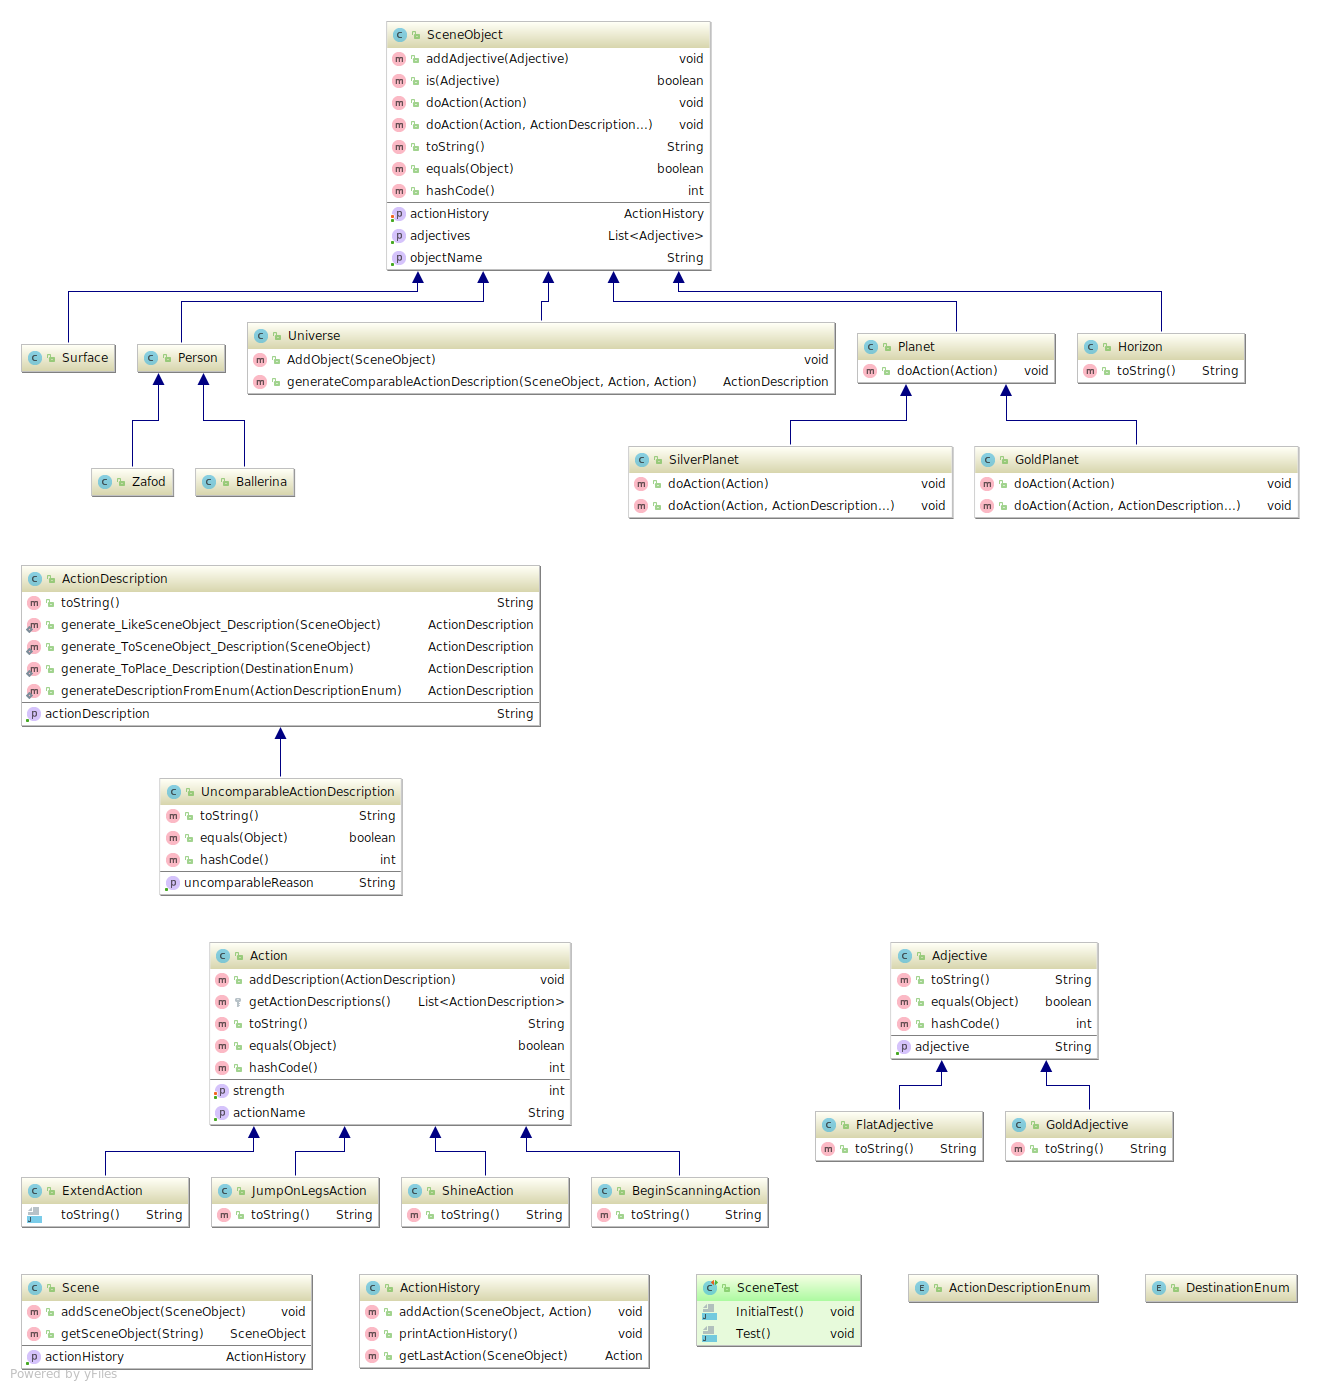
\includegraphics[scale=0.35]{scene_uml.png}
\subsection{Исходный код}
Не будем приводить полный исходный код, так как это не будет иметь смысла - очень много классов имеют схожий код внутри.
\subsubsection{SceneObject.java}
\lstinputlisting[language=java]{../src/main/java/testing/lab1/scene/SceneObject.java}
\subsubsection{Action.java}
\lstinputlisting[language=java]{../src/main/java/testing/lab1/scene/Action.java}
\subsubsection{ActionHistory.java}
\lstinputlisting[language=java]{../src/main/java/testing/lab1/scene/ActionHistory.java}
\subsubsection{Scene.java}
\lstinputlisting[language=java]{../src/main/java/testing/lab1/scene/Scene.java}
\subsection{Тесты}
% Приколы с юникодом, сорян
\begin{lstlisting}[language=java]
package testing.lab1.scene;

import org.junit.Test;

import static junit.framework.TestCase.assertNotNull;
import static junit.framework.TestCase.assertTrue;

public class SceneTest {

	@Test
	public void InitialTest() {
		Scene scene = new Scene();
		
		SceneObject obj1 = new SceneObject("obj1");
		SceneObject obj2 = new SceneObject("obj2");
		
		Action act1 = new Action("act1");
		Action act2 = new Action("act2");
		
		scene.addSceneObject(obj1);
		scene.addSceneObject(obj2);
		
		obj2.doAction(act1);
		obj1.doAction(act2);
		
		scene.getActionHistory().printActionHistory();
		
		assert(act1.getActionName().equals("act1"));

	}

	@Test
	public void Test() {
		//this has all the magic happening
		Scene scene = new Scene();
		
		//creating zafod and balerina
		Zafod zafod = new Zafod();
		Ballerina ballerina = new Ballerina();
		
		//this makes zafod log his actions to scene's log
		scene.addSceneObject(zafod);
		
		JumpOnLegsAction jump = new JumpOnLegsAction();
		zafod.doAction(jump, ActionDescription.generateDescriptionFromEnum(ActionDescriptionEnum.easily), ActionDescription.generate_LikeSceneObject_Description(ballerina));
		Action a = zafod.getActionHistory().getLastAction(zafod);
		assertTrue(a instanceof JumpOnLegsAction 
		&& a.getActionDescriptions().stream().anyMatch(
		ad -> ad.getActionDescription().equals("easily")));
		
		zafod.doAction(new BeginScanningAction());
		a = zafod.getActionHistory().getLastAction(zafod);
		assertTrue(a.getActionName().contains("scanning"));
		
		Surface surface = new Surface();
		scene.addSceneObject(surface);
		assertNotNull(scene.getSceneObject("surface"));
		
		Horizon horizon = new Horizon();
		ExtendAction extend = new ExtendAction();
		GoldAdjective ga = new GoldAdjective();
		FlatAdjective fa = new FlatAdjective();
		
		surface.addAdjective(ga);
		surface.addAdjective(fa);
		surface.doAction(extend, ActionDescription.generate_ToSceneObject_Description(horizon), ActionDescription.generate_ToPlace_Description(DestinationEnum.all_sides));
		assertTrue(
			surface.getActionHistory().getLastAction(surface)
			.getActionDescriptions().stream().anyMatch(
			ad -> ad.getActionDescription().contains(
			horizon.getObjectName()))
			&&
			surface.getActionHistory().getLastAction(surface)
			.getActionName().equals(
			new ExtendAction().getActionName())
			&&
			surface.is(new GoldAdjective())
			&&
			surface.is(new FlatAdjective())
		);
		
		
		//class universe with silver planet to compare shining strength to
		Universe uni = new Universe();
		SilverPlanet sp = new SilverPlanet();
		uni.AddObject(sp);
		
		
		ShineAction shine = new ShineAction();
		shine.setStrength(GoldPlanet.SHINING_STRENGTH);
		
		surface.doAction(shine, uni.generateComparableActionDescription(new GoldPlanet(), shine, new ShineAction()));
		assertTrue(surface.getActionHistory().getLastAction(surface).
		getActionDescriptions().stream().
		anyMatch(ad -> ad instanceof UncomparableActionDescription));
		
		//print out the whole story
		scene.getActionHistory().printActionHistory();
		
		//TODO: loads of more useful asserts
		assert(zafod.getObjectName().equals("Zafod"));
	}
}
\end{lstlisting}

\section{Выводы}
В ходе выполнения данной лабораторной работы было создано некоторое количество программных модулей, а также проведено тестирование разработанных модулей с использование средств JUnit4.


\end{document}
